\section{Encode Experiments} \label{integr-encode-exper-sect}
To evaluate the performance of the BCC model, we will use the same ENCODE datasets that were described in \emph{Section \ref{encode-data-sect}}, that is, the RRBS and RNA-Seq data produced from K562 and H1-hESC cell lines.

\subsection{Data Processing}
The procedure for preprocessing the raw experimental data and defining promoter regions is exactly the same as described in \emph{Section \ref{meth-encode-experiments-sect}}. 

To perform integrative clustering we have to define the different data sources $m$ and the observation models $f_{m}(X_{mn}|\theta_{m})$ that each data source follows. For our experiments we have two data sources, RNA-Seq and RRBS, for a common set of N objects, where as objects we define the different protein-coding genes.

RNA-Seq experiments return count based measure of gene expression and a natural choice to statistically model these data is a \emph{Poisson} observation model. Thus, we assume that each object from the RNA-Seq data source is generated from a Poisson mixture distribution:
\begin{equation}
	X_{mn} \mid L_{mn} = k, \theta_{mk} \sim \mathcal{P}ois\big(\lambda_{mk}\big)
\end{equation}

The measurement process of DNA methylation from RRBS experiments can be modelled with a Binomial distribution, that is, each CpG site follows a Binomial distribution. Since, our objects are protein-coding genes, it does not make sense to model each CpG site, but rather we should consider promoter regions and model the methylation level of these regions. A promising approach for this problem would be to model each methylation profile using the \emph{Binomial distributed Probit regression} function introduced in \emph{Chapter \ref{model-meth-chapter}}. Even though this model is promising, it cannot be integrated in the BCC model in a straightforward way, as it is  explained in \emph{Section \ref{conc-meth-prof-bcc-subsect}}.

Hence, in order to evaluate the RRBS data with the BCC model, we take a crude approach by summing the methylation level of all the CpGs in each promoter region. Assuming \emph{independence} of the methylation level between CpG sites, the sum of independent Binomial random variables will also follow a Binomial distribution. Thus, we assume that each object from the RRBS data source is generated from a Binomial mixture distribution:
\begin{equation}
	X_{mn} \mid L_{mn} = k, \theta_{mk} \sim \mathcal{B}inom\big(t_{mk}, \rho_{mk}\big)
\end{equation}

The independence assumption is a strong assumption, since the the methylation level of a CpG site is highly correlated with the methylation level of the surrounding CpGs (i.e. spatial co-dependence). Also, by summing the methylation level of the CpGs in each region and representing each promoter with a single methylation value we discard  important features of the data. For example, methylation profiles with low methylation upstream of TSS and high methylation downstream of TSS, would have similar methylation value with their reverse pattern, that is, methylation profiles with high methylation upstream of TSS and low methylation downstream of TSS. These issues, need to be understood and taken into consideration when analysing the results of the BCC model.

\subsection{Evaluation}
To evaluate the performance of the BCC model on these real datasets, we decided to concatenate the different experiments conducted on each cell line, resulting in 2-dimensional datasets for each data source. That is, for the RRBS data source, the $1^{st}$ dimension will be the experiments for the K562 cell line and in the $2^{nd}$ dimension the ones for the H1-hESC cell line. Similarly for the RNA-Seq data source.

After pre-processing each dataset individually, we mapped the TSS of the genes from both datasets. This procedure resulted in 604 protein-coding genes for testing. The total number of MCMC iterations was set to $T=20,000$ and the first $5,000$ iterations were discarded, \ie burn-in period. The total number of clusters K was set to 3. This was an empirical choice, since a bigger number would result in empty clusters or clusters with only a few objects assigned to them. 

\emph{Figure \ref{bcc2D-pic}} provides scatter plots of the datasets for the RRBS source (ME) and the RNA-Seq source (GE), together with the adherence parameter value $\alpha$. Each point depicts a different 2-dimensional object, where the \emph{x-axis} is the K562 cell line and the \emph{y-axis} is the H1-hESC cell line. Each object is coloured according the overall clustering assignment; cluster 1 is black, cluster 2 is red and cluster 3 is blue. The symbols indicate source-specific clusterings; filled circles for cluster 1, plus signs for cluster 2 and asterisks for cluster 3. 

\begin{figure}[ht!]
     \begin{center}
        \subfigure[]{
            \label{bccME2D:first}
            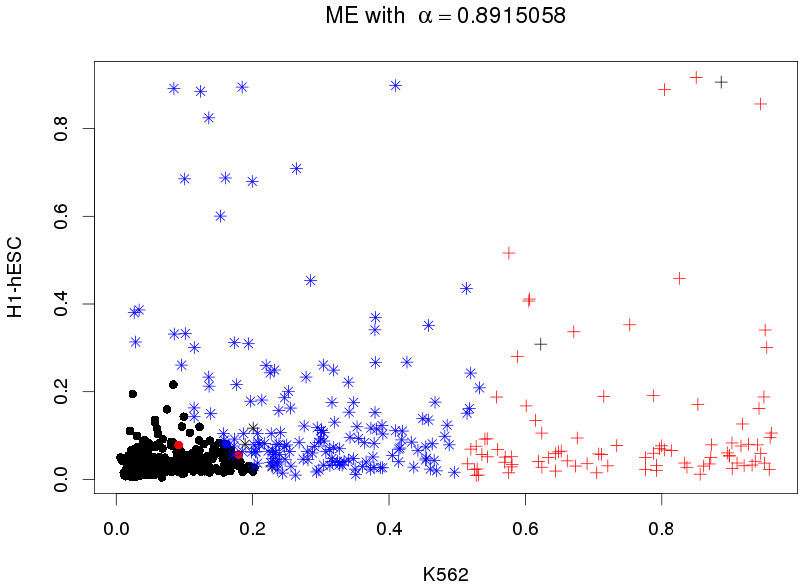
\includegraphics[width=0.48\textwidth]{images/bccME2D-2}
        }
        \subfigure[]{
           \label{bccGE2D:second}
           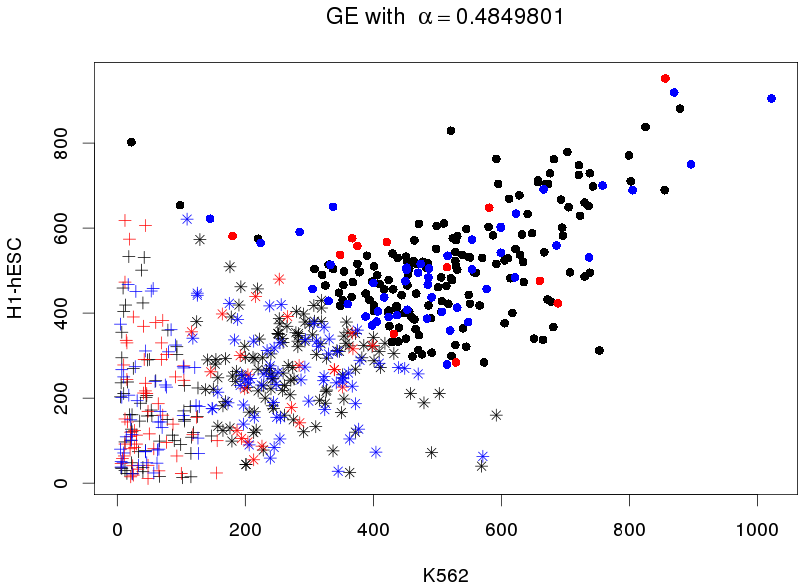
\includegraphics[width=0.48\textwidth]{images/bccGE2D-2}
        }
    \end{center}
    \caption{\emph{Scatter plots for each data source; (a) RRBS source and (b) RNA-Seq source.  Each object is coloured according the overall clustering assignment; cluster 1 is black, cluster 2 is red and cluster 3 is blue. The symbols indicate source-specific clusterings; filled circles for cluster 1, plus signs for cluster 2 and asterisks for cluster 3. See the text for details.}}
   \label{bcc2D-pic}
\end{figure}


\begin{figure}[ht!]
     \begin{center}
        \subfigure[]{
            \label{bccMEMV:first}
            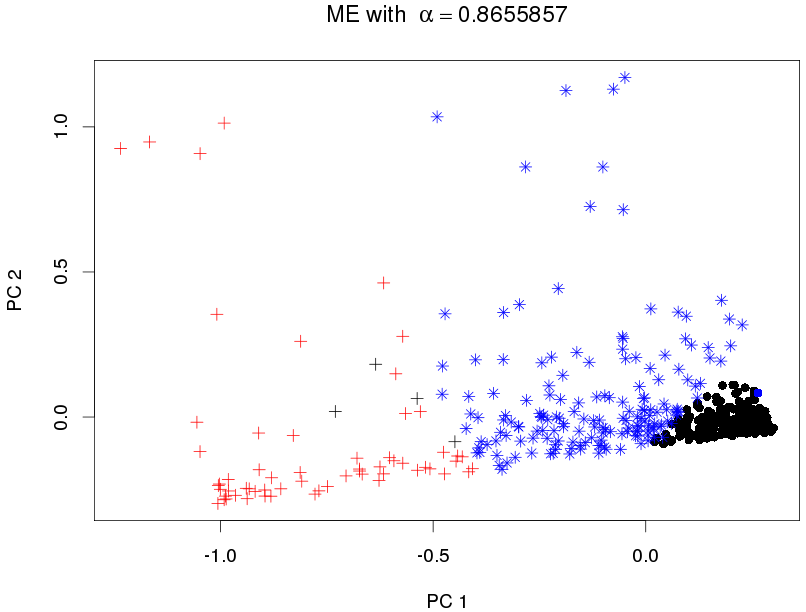
\includegraphics[width=0.48\textwidth]{images/bccMEMV-2}
        }
        \subfigure[]{
           \label{bccGEMV:second}
           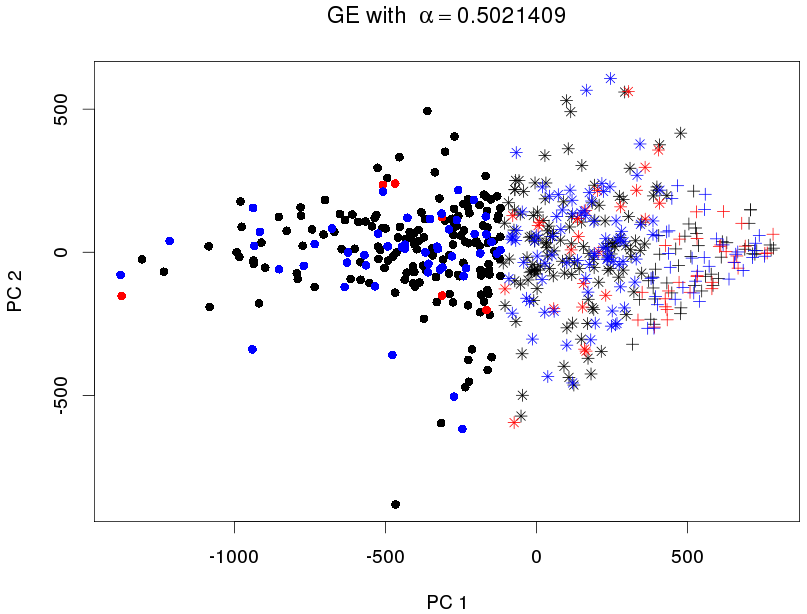
\includegraphics[width=0.48\textwidth]{images/bccGEMV-2}
        }
    \end{center}
    \caption{\emph{Scatter plots for each data source for both replicates of the K562 cell line; (a) RRBS source and (b) RNA-Seq source.  Each object is coloured according the overall clustering assignment; cluster 1 is black, cluster 2 is red and cluster 3 is blue. The symbols indicate source-specific clusterings; filled circles for cluster 1, plus signs for cluster 2 and asterisks for cluster 3. See the text for details.}}
   \label{bccMV-pic}
\end{figure}


\subsection{K562 cell line}
Both RRBS and RNA-Seq experiments for the K562 cell line contain two technical replicates. Thus, for the evaluation of the BCC model we decided to concatenate the replicates, resulting in 2-dimensional datasets. After pre-processing each replicate individually, we mapped the TSS of the genes from both replicates. This procedure resulted in 978 protein-coding genes for testing. The total number of MCMC iterations was set to $T=20,000$ and the first $5,000$ iterations were discarded, \ie burn-in period. For the experiments we selected K=3 clusters. This was an empirical choice for this dataset, since a bigger number would result in empty clusters or clusters with only a few objects assigned to them.

\begin{figure}[ht!]
     \begin{center}
        \subfigure[]{
            \label{bccMEk562:first}
            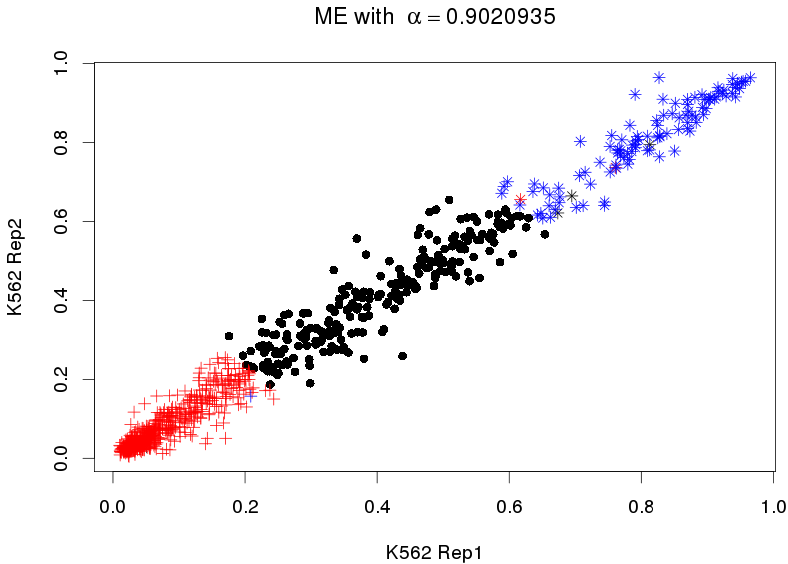
\includegraphics[width=0.48\textwidth]{images/bccMEk562-2}
        }
        \subfigure[]{
           \label{bccGEk562:second}
           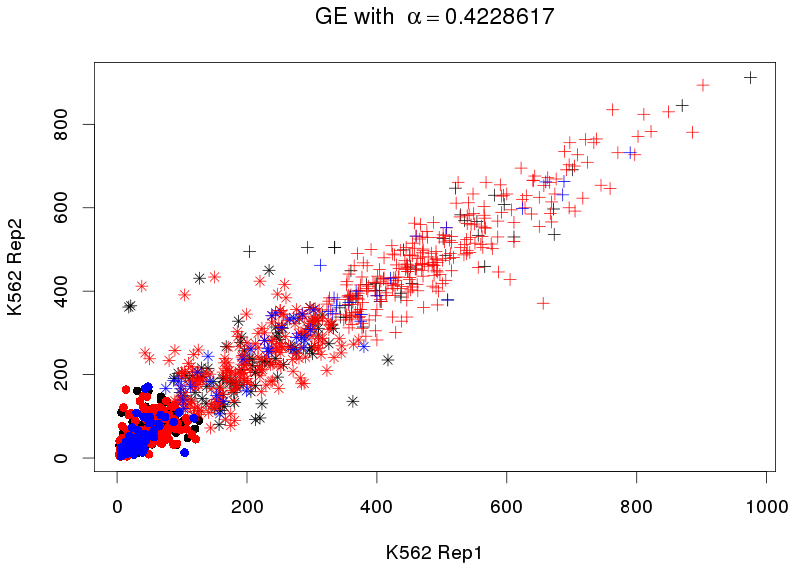
\includegraphics[width=0.48\textwidth]{images/bccGEk562-2}
        }
    \end{center}
    \caption{\emph{Scatter plots for each data source for both replicates of the K562 cell line; (a) RRBS source and (b) RNA-Seq source.  Each object is coloured according the overall clustering assignment; cluster 1 is black, cluster 2 is red and cluster 3 is blue. The symbols indicate source-specific clusterings; filled circles for cluster 1, plus signs for cluster 2 and asterisks for cluster 3. See the text for details.}}
   \label{bcck562-pic}
\end{figure}


 We argue that this behaviour may be related with our approach in summing the methylation level of all CpGs in each promoter region, since 

